% !TEX root = ../../../main.tex
% 来源：中学数学实验教材·第三册（高中数学）
% 章节：函数及其图象 / 一次函数（线性函数）
% 原始文件：4.tex，行 2466-2511
% 类型：tikz
% ---
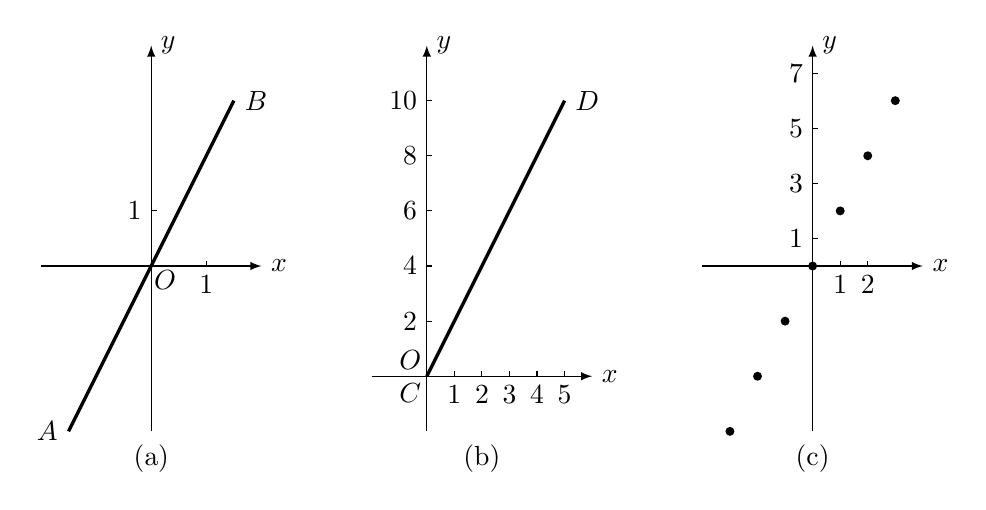
\begin{tikzpicture}[>=latex, scale=.7]
\begin{scope}
    \draw[->] (-2,0) --(2,0)node[right]{$x$};
    \draw[->] (0,-3)--(0,4)node[right]{$y$};
    \draw[very thick](-1.5,-3)node[left]{$A$}--(1.5,3)node[right]{$B$};
    \draw (0,1)node[left]{1}--(.1,1);
    \draw (1,0)node[below]{1}--(1,.1);
    \node at (.25,-.25){$O$};

    \node at (0,-3.5){(a)};
\end{scope}
\begin{scope}[xshift=5cm, yshift=-2cm]
    \draw[->] (-1,0) --(3,0)node[right]{$x$};
    \draw[->] (0,-1)--(0,6)node[right]{$y$};
    \draw[very thick](0,0)--(2.5,5)node[right]{$D$};
\foreach \x in {1,2,...,5}
{
    \draw(\x/2,0)node[below]{$\x$}--(\x/2,.1);
}
\foreach \x in {2,4,...,10}
{
    \draw (0,\x/2)node[left]{$\x$}--(.1,\x/2);
}
\node at  (-.3,-.3){$C$};
\node at  (-.3,.3){$O$};
\node at (1,-1.5){(b)};
\end{scope}
\begin{scope}[xshift=12cm]
    \draw[->] (-2,0) --(2,0)node[right]{$x$};
    \draw[->] (0,-3)--(0,4)node[right]{$y$};
    \foreach \x in {1,2}
    {
        \draw(\x/2,0)node[below]{$\x$}--(\x/2,.1);
    }
    \foreach \x in {1,3,5,7}
    {
        \draw (0,\x/2)node[left]{$\x$}--(.1,\x/2);
    }
\foreach \x in {-3,-2,...,3}
{
    \draw (\x/2,\x) [fill=black] circle(2pt);
}
\node at (0,-3.5){(c)};
\end{scope}

\end{tikzpicture}
